\documentclass[11pt]{article}
\usepackage[margin=1in]{geometry}
\usepackage[T1]{fontenc}
\usepackage{lmodern,microtype,amsmath,amssymb,graphicx,booktabs,tabularx,array}
\usepackage{enumitem}
\usepackage[hidelinks]{hyperref}
\usepackage{xurl}
\usepackage{caption}
\usepackage{placeins}
\captionsetup{font=small,labelfont=bf}
\setlength{\parskip}{3pt}
\setlength{\parindent}{1.2em}
\setlength{\emergencystretch}{3em}
\setlist{nosep,topsep=4pt}
\newcolumntype{Y}{>{\raggedright\arraybackslash}X}
\newcommand{\takeaway}[1]{\par\noindent\textbf{Current conclusion.} #1\par}
\newcommand{\prompt}[2]{\par\noindent\textbf{#1}\begin{quote}\small\raggedright\ttfamily #2\end{quote}}
\graphicspath{{notes_figures/}}
\title{Do CoVT's Depth Visualizations Reflect\\the Information Used to Answer?\\[4pt]\large Research Notes on Model Principles, Pilot Experiments, and Causal Tests}
\author{}
\date{September 18, 2026}
\hypersetup{pdftitle={Do CoVT's Depth Visualizations Reflect the Information Used to Answer?},pdfsubject={CoVT background, pilot experiments, and revised research plan}}
\begin{document}
\maketitle
\begin{abstract}
We study Chain-of-Visual-Thought (CoVT), a visual language model that can expose intermediate visual representations. Our question is simple: when a model's depth visualization correctly identifies the nearer object, does the model use that information to produce its answer? These notes explain the model, reproduce the actual question prompts, and consolidate the first proposal with completed pilot experiments. The recovered visualization depends strongly on image features supplied by a depth expert: even fixed CoVT states often produce correct depth relations. In contrast, replacing selected internal states across individual layers, layer blocks, and all layers has not changed the generated answers in the tested settings. These results motivate targeted information-path analysis. They do not yet identify a faulty answer reader or establish that visual states are universally unused. No repair training has been completed.
\end{abstract}

\section{What is CoVT, and what are we trying to understand?}
A \emph{visual language model} (VLM) receives an image and a text question, then generates text. For example, it may receive a picture with two labeled balls and answer ``B'' to ``Which is closer?'' Internally, the picture and question are represented by arrays of numbers. Repeated computation updates these arrays before the model predicts its next output symbol.

\textbf{CoVT stands for Chain-of-Visual-Thought}~\cite{covt}. Our current experimental subject is its released depth version. The model and training method belong to the original authors; the controlled tests described here are our investigation.

Ordinary text reasoning produces intermediate words. CoVT additionally generates special positions whose numerical representations are trained to relate to visual properties. A separate visualization computation can turn these representations, together with expert image features, into a depth map. A depth map assigns each image location a score associated with distance. Its colors are a display convention, not measured meters.

Our motivating observation is that the map can indicate B while the text answer says A. This is an observable disagreement, but its cause is not self-evident. The map may receive most of its useful information from the expert. The answer may use other image information. Or the two computations may respond differently to the same internal information. We want to distinguish these possibilities experimentally.

\textbf{Why this matters.} A correct intermediate picture can make an answer seem well supported. To use that picture as an explanation, we need to know how it relates to the calculation that produced the answer. Establishing this relation also tells us whether a future improvement should target visual representation, answer computation, or their connection. The intended contribution is an explicit, reproducible account of this relation, followed by a limited repair only if the mechanism warrants one.
\takeaway{A correct depth picture establishes that a particular visualization procedure can recover a relation. By itself, it does not establish that the model used that relation when answering.}

\section{How CoVT works}
\subsection{From an image to visual states and an answer}
A \emph{token} is an input or output position processed by the model. Tokens can represent pieces of text, special control symbols, or image-related content. A \emph{hidden state} is the vector of numbers at one position and one processing layer. It changes as the model computes. A \emph{decoder} here means the additional computation used to produce a visible map; it should not be confused with the whole language model.

Figure~\ref{fig:overview} shows how CoVT interleaves text and visual-token positions before producing an answer. The visual thought is a numerical representation. The displayed map is a later interpretation of that representation using a particular readout procedure.
\begin{figure}[htbp]\centering
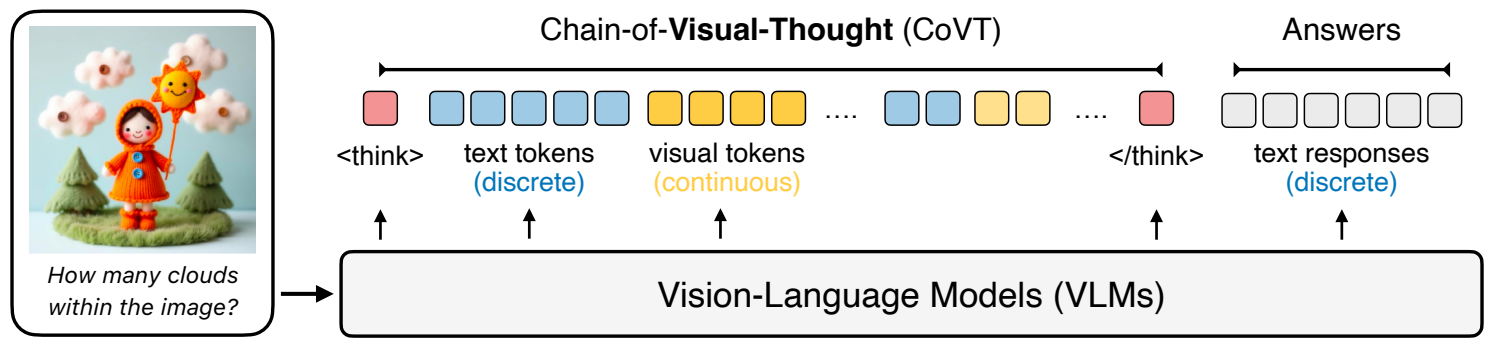
\includegraphics[width=\linewidth]{paper_1.png}
\caption{Overview reproduced from Fig.~1 of the CoVT paper~\cite{covt}. Read from left to right: an image enters the VLM, text and visual tokens form an intermediate sequence inside the thought tags, and the model produces an answer. Colored token blocks distinguish token types; they are not measured depth values or accuracy scores. This is the authors' method illustration, not a result of our pilot.}\label{fig:overview}
\end{figure}

We use \texttt{Wakals/CoVT-7B-depth}, built on Qwen2.5-VL. In the audited depth path, four generated \texttt{<|depth\_pad|>} positions provide four states. Each state has 3,584 components. These are not four objects or four hand-defined categories such as near, far, foreground, and background. Their learned roles are determined by training and by the downstream calculation.

\subsection{What the depth expert contributes}
The \emph{depth expert} is a separate pretrained vision system. In this implementation, the expert uses a DINOv2 ViT-L backbone and a DPT depth head associated with Depth Anything V2~\cite{dav2}. The backbone produces spatial features: at each grid location it stores a vector describing image content. The depth head combines such features into a relative-depth prediction. The expert prediction can be wrong and is never used as our ground-truth label.

The important detail is that CoVT's displayed depth map uses both the four CoVT states and expert features computed from the original image. Figure~\ref{fig:readout} shows examples of the visual outputs the original authors expose. Therefore, the displayed map is a \emph{conditional readout}: its information can come from both inputs.
\begin{figure}[htbp]\centering
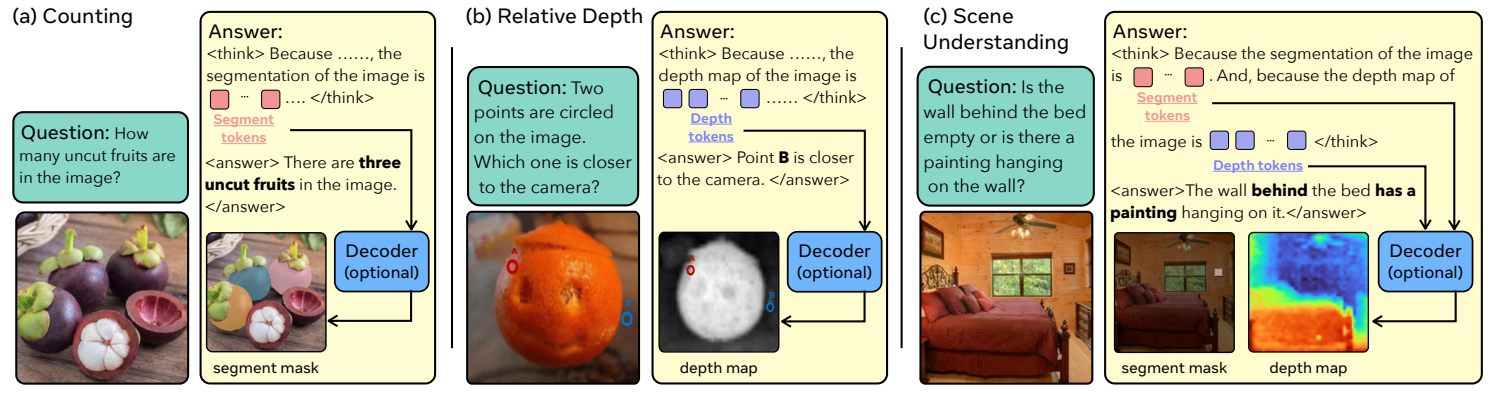
\includegraphics[width=\linewidth]{paper_2.png}
\caption{Task examples reproduced from Fig.~2 of the CoVT paper~\cite{covt}: counting, relative depth, and scene understanding. The panels pair images with intermediate visualizations and answers. The middle panel illustrates the kind of depth output investigated here. Colors distinguish visual outputs and text boxes; there are no numerical axes. These examples show what can be displayed, not which input contributes the information.}\label{fig:readout}
\end{figure}

For the restored code path, write the four states as $H=(h_1,\ldots,h_4)$ and the expert feature grids as $F=(F_1,\ldots,F_4)$. A learned projection converts each $h_i$ to a 1,024-component vector:
\begin{align}
 t_i &= W_2\,\mathrm{GELU}(W_1 h_i+b_1)+b_2,\\
 M_i(p)&=\sum_{c=1}^{1024} t_{i,c}F_{i,p,c},\qquad
 D=\frac14\sum_{i=1}^{4}\operatorname{Resize}(M_i).
\end{align}
Here $p$ is a spatial grid location and $c$ indexes vector components. GELU is a fixed nonlinear transformation inside the small projection network. The expert grids come from backbone blocks 4, 11, 17, and 23, each on a $37\times37$ grid. The four maps are resized to the decoder grid and averaged. We use 256-pixel decoder maps and aligned $336\times336$ maps for scoring.

In plain terms, a CoVT state supplies weights and the expert supplies image-dependent spatial information. Even constant weights may recover a useful map when the expert features already organize distance well. This is the reason for our fixed-state control. The restored released computation uses the dot products above without a spatial softmax; the paper's displayed formulation includes softmax. We document the implementation we actually evaluated rather than silently treating these as identical.

\subsection{Training, answering, and visualizing are different operations}
During training, expert-derived visual supervision encourages the special states to represent visual properties. Figure~\ref{fig:training} illustrates the original training framework. During ordinary answer generation, the language model processes the image, question, and generated sequence. Running an external expert to render a map for our inspection is a separate operation; it is not required to be on the answer-generation path.
\begin{figure}[htbp]\centering
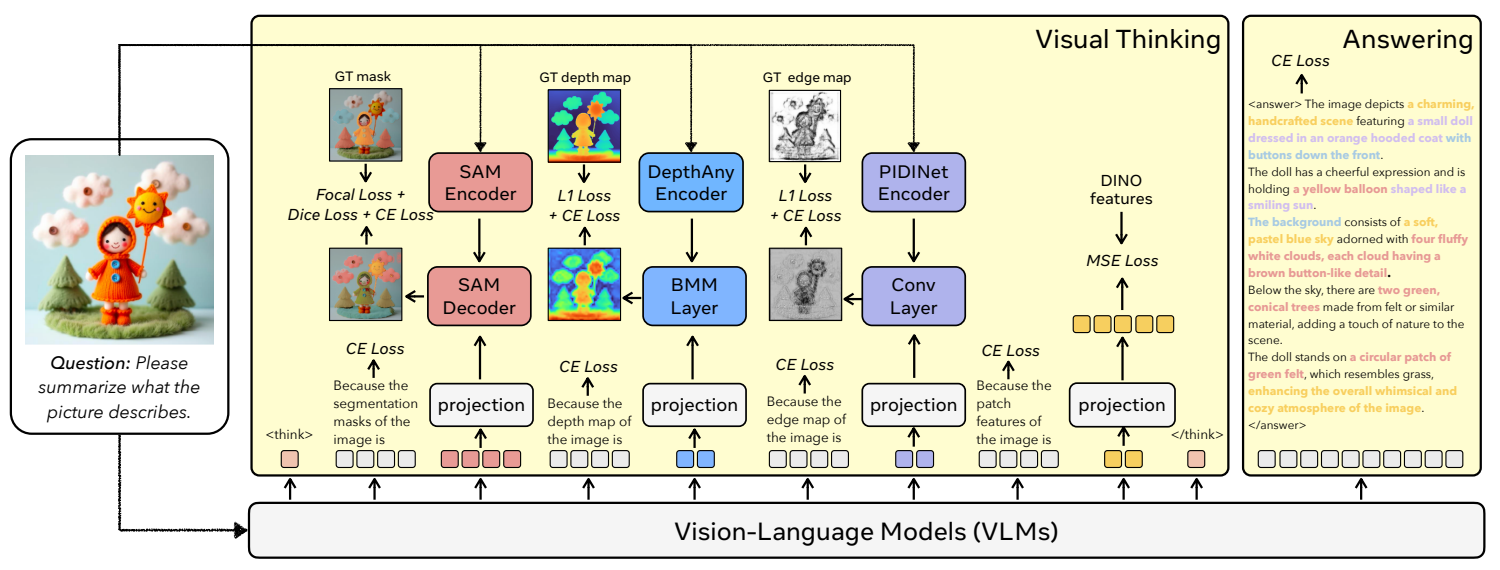
\includegraphics[width=\linewidth]{paper_3.png}
\caption{Training illustration reproduced from Fig.~3 of the CoVT paper~\cite{covt}. The diagram shows how the original method connects visual supervision and model training. Arrows describe training information flow, not proof that every displayed map causally determines an inference-time answer. Our pilot restores a released checkpoint; it does not repeat this training.}\label{fig:training}
\end{figure}
\takeaway{Four states can participate in a useful visualization without each having a known human-readable meaning. Training supervision, map reconstruction, and answer generation must be tested separately.}
\FloatBarrier

\section{Task, data, and exact prompts}
\subsection{What is in the dataset?}
We use rendered scenes because their geometry gives an independent answer. Two visible surface points are marked A and B. Their camera-axis depths are $z_A$ and $z_B$; the correct answer is A if $z_A<z_B$, otherwise B. This is distance along the camera axis, not Euclidean distance to the camera center. The scene units are not calibrated meters.

A \emph{scene family} groups related variants generated from one underlying scene. Variants can change depth order, color, or label assignment. Related images are useful controls, but do not count as independent scenes. Table~\ref{tab:data} lists the four archived batches. Their 284 image records form 71 families; prompt variants and repeated interventions do not add independent images to this count.
\begin{table}[htbp]\centering\small
\begin{tabularx}{\linewidth}{lrrY}\toprule
Batch & Images & Families & Purpose\\\midrule
Initial restoration &12&3&4 calibration images; 8 pilot images.\\
FP32 follow-up &40&10&8 calibration images; 32 evaluation images.\\
Geometry shifts &200&50&40 images each: size, ellipsoid, box, occlusion, camera changes.\\
Size-balanced &32&8&Cross nearer label with apparent-size agreement, four variants per family.\\\bottomrule
\end{tabularx}\caption{Archived base-image records, not counts of model runs. Subsequent tests reuse subsets of these batches.}\label{tab:data}
\end{table}
\begin{figure}[htbp]\centering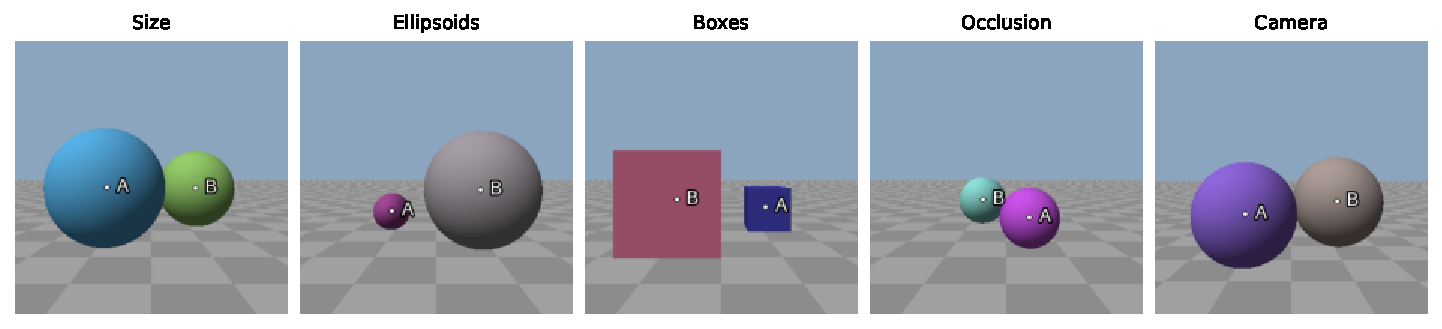
\includegraphics[width=\linewidth]{dataset.pdf}
\caption{Actual images from the geometry-shift batch. Left to right: size variation, ellipsoids, boxes, partial occlusion, and camera variation. A and B mark the queried visible surface points. These are examples of the five strata, not five independent test sets beyond the 200-image batch. No numerical axes are used.}\label{fig:data}
\end{figure}

Figure~\ref{fig:case} gives a concrete example. In archived scene \texttt{scene\_00002\_base}, $z_A\approx5.37954$ and $z_B\approx3.40779$, so B is nearer by construction. A is marked at pixel $(222,191)$ and B at $(113,201)$. B also appears larger in this example, but size is not how we assign the answer. Later experiments deliberately separate apparent size from depth.
\begin{figure}[htbp]\centering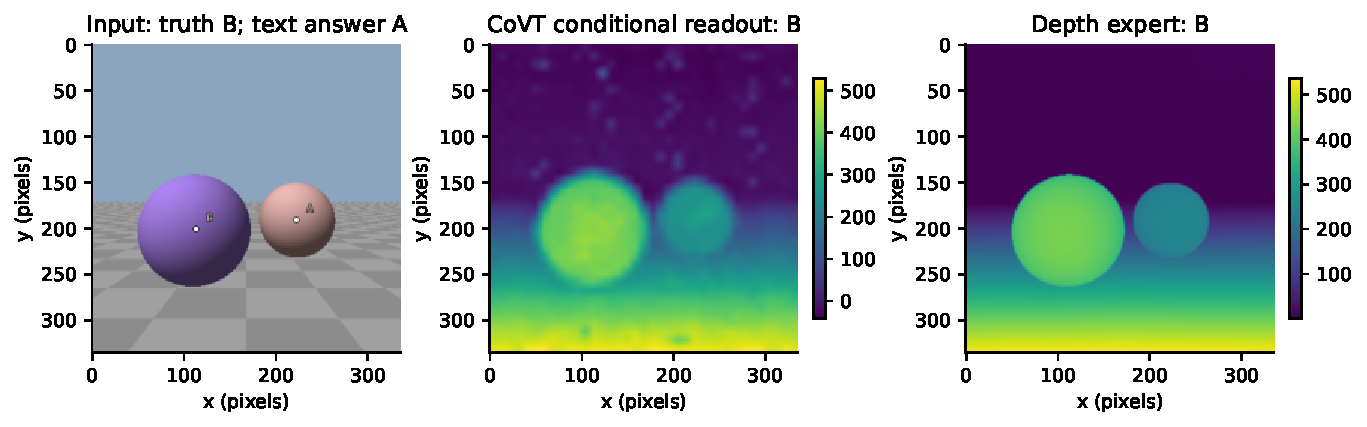
\includegraphics[width=\linewidth]{native_case.pdf}
\caption{An actual motivating failure. Left: input image, ground truth B, generated text answer A. Middle: reconstructed CoVT map; right: expert map. Both maps yield B under the calibrated relation rule. Horizontal axes are image columns $x$; vertical axes are rows $y$, increasing downward. Color bars show raw readout scores, not meters; each map has its own color scale. Numerical colors cannot be compared directly across panels.}\label{fig:case}
\end{figure}

\subsection{What exactly did we ask the model?}
The following strings are copied from the experiment code. Each user message contains the marked image followed by the question text. The checkpoint processor applies its chat template and adds the assistant-generation prefix. We do not manually insert four depth states to force a successful extraction. Original runs use deterministic generation (\texttt{do\_sample=False}); the restoration wrapper defaults to at most 192 new tokens. Per-run configuration remains authoritative.

\prompt{Original technical wording}{Which marked surface point, A or B, has smaller camera-axis depth (closer to the image plane)? Answer A or B.}
This is used in the original synthetic batch. It expresses the geometric target precisely, but may be harder to interpret than ordinary language.

\prompt{Plain near question}{Which marked point is closer to the camera, A or B? Answer only A or B.}
This asks the same intended ordering in simpler language and is also used for the later geometry-shift scenes. On the example above, the expected answer is B. This is an expected label, not a claim that the model actually returned B for every prompt variant.

\prompt{Far question}{Which marked point is farther from the camera, A or B? Answer only A or B.}
The expected label reverses: A in the example. Asking both near and far tests whether the answers are mutually consistent.

\prompt{Label-reading control}{Which label is on the left side of the image, A or B? Answer only A or B.}
This checks whether the model can identify the letter and its location. In the example the answer is B, independently of the depth question.

\prompt{Apparent-size control}{Which labeled sphere occupies more area in the image, A or B? Answer only A or B.}
This asks about projected image area, not physical size or depth. The expected label is obtained from rendered object masks.

\prompt{Alternative answer vocabulary}{Which sphere is closer to the camera, the left sphere or the right sphere? Answer only left or right.}
This reduces reliance on mapping depth to the letters A and B. Two additional conditions reuse the plain-near and label-reading prompts on images with enlarged letters. Together these give eight diagnostic tasks, evaluated on 16 images from eight families for each of two models: $8\times16\times2=256$ runs.

Answers are parsed from the model's final answer field where present, with explicit handling for simple A/B forms. Ambiguous ``A or B'', truncated answers, and broken output tags are recorded separately. A prompt that requests one letter does not guarantee that the checkpoint omits its usual intermediate output.
\takeaway{The data let us vary geometry and labels separately. The prompt controls distinguish depth ordering, label reading, apparent size, and output vocabulary; success on one task does not establish success on another.}
\FloatBarrier

\section{How we measure the two outputs}
\textbf{Depth relation.} At each marker we sample an annulus with inner radius 5 and outer radius 9 pixels, reducing contamination from the printed letter. Let $a$ and $b$ be the median raw map scores in the A and B annuli. Calibration-only images determine a sign $s\in\{-1,1\}$ and scale $c=\operatorname{median}|b-a|$ over nonzero calibration differences. The sign is chosen so positive normalized differences correspond to A on calibration labels. A tied direction or flat calibration map is a failure. We then freeze
\begin{equation}
 r=s(b-a)/c,\qquad
 \widehat y_D=\begin{cases}A&r>0.05,\\B&r<-0.05,\\\text{abstain}&|r|\leq0.05.\end{cases}
\end{equation}
This gives each map a relation prediction without asking another language model to judge its colors. As an illustrative calculation, $s=-1$, $c=100$, and $b-a=-80$ give $r=0.8$ and label A. A difference of $-3$ gives $r=0.03$, so the readout abstains. These numbers illustrate the formula and are not another experimental sample.

\textbf{Answer behavior.} We report text correctness, format validity, and answer changes separately. A valid answer flip requires two unambiguous answers. We also inspect the answer-token probability
\begin{equation}
 q_A=\frac{\exp(\ell_A)}{\exp(\ell_A)+\exp(\ell_B)},\qquad
 \Delta q_A=q_A^{\mathrm{intervention}}-q_A^{\mathrm{baseline}},
\end{equation}
where $\ell_A,\ell_B$ are the corresponding logits at the audited answer position. The A/B-normalized probability is conditional on this pair of alternatives; it is not the probability that the whole response is well formed. A change of $0.0005$ is $0.05$ percentage points, not a five-percent answer flip rate.

\textbf{Statistical unit.} Image accuracy is correct images divided by evaluated images, with abstentions reported. For a family mean, we first average within each family and then give each family equal weight. Reported exploratory intervals use 2,000 bootstrap resamples of families with seed 0 and the 2.5th and 97.5th percentiles. Repeating a shuffle with five seeds does not multiply the number of independent families. Few-family intervals can be unstable or degenerate.
\takeaway{A good map, a correct answer, a valid output format, and a small probability shift measure different things. We keep their denominators and interpretations separate.}

\section{Completed pilot experiments}
The following experiments use restored checkpoints and archived Colab runs. No training was performed. The first proposal called restoration E0 and decoder-input decomposition E1; later experiments below are additional completed controls, not evidence that all original E0--E5 stages are finished.

\subsection{Restoring the native readout (E0)}
\textbf{Purpose and design.} Before interpreting a map, verify that the checkpoint, projection parameters, token positions, and replay procedure are recovered correctly. We compare generation with and without the key/value cache, which stores intermediate computations for faster generation. Replay extracts the states at the actual generated depth-pad input positions after the final language normalization. We do not shift them to neighboring positions or silently select four tokens from an invalid sequence.

\textbf{Example.} If cached and uncached generation disagree near an A/B decision boundary, an apparent mechanism change may instead be a numerical difference. A controlled precision check is needed before interpreting the answer.

\textbf{Results.} In the initial 12-image BF16 batch, two examples failed the cache-consistency audit. Seven of eight pilot images were eligible for the reported joint comparison: the depth relation was correct on 7/7 and the text answer on 2/7. A targeted precision comparison motivated FP32 follow-up, where all 40 examples passed the restoration checks. On its 32 evaluation images, depth was correct on 32/32 and text on 8/32. The precise source of the BF16 discrepancy has not been localized; a successful FP32 run alone does not identify it.
\takeaway{We recovered a usable native readout for the audited FP32 batch. The map--answer gap is real in that batch, but its mechanism remains open.}

\subsection{Separating CoVT states from expert image features (E1)}
\textbf{Purpose and design.} Determine which input carries the observed depth-order change into the visualization. For paired scenes 0 and 1, evaluate all four combinations $D(H_0,F_0)$, $D(H_1,F_0)$, $D(H_0,F_1)$, and $D(H_1,F_1)$. Only one input changes at a time. Define state and feature effects on the calibrated relation score as
\begin{equation}
 \delta_H=r(H_1,F_0)-r(H_0,F_0),\qquad
 \delta_F=r(H_0,F_1)-r(H_0,F_0).
\end{equation}
\textbf{Example.} Scene 0 has A nearer and scene 1 has B nearer. Substituting $H_1$ keeps the expert's view of scene 0. Substituting $F_1$ changes the expert's view while keeping scene 0's state. The decoder output shows which substitution transfers the relation.

\textbf{Results.} Across eight depth-swap pairs, state-only substitution changed the readout label in 0/8 cases; feature-only substitution changed it in 8/8. Mean absolute relation-score changes were approximately 0.000311 and 1.802808, respectively (Fig.~\ref{fig:factorial}). Color-only changes provide a nuisance comparison. These operations modify the visualization inputs after state extraction; they are not interventions on answer generation.
\begin{figure}[htbp]\centering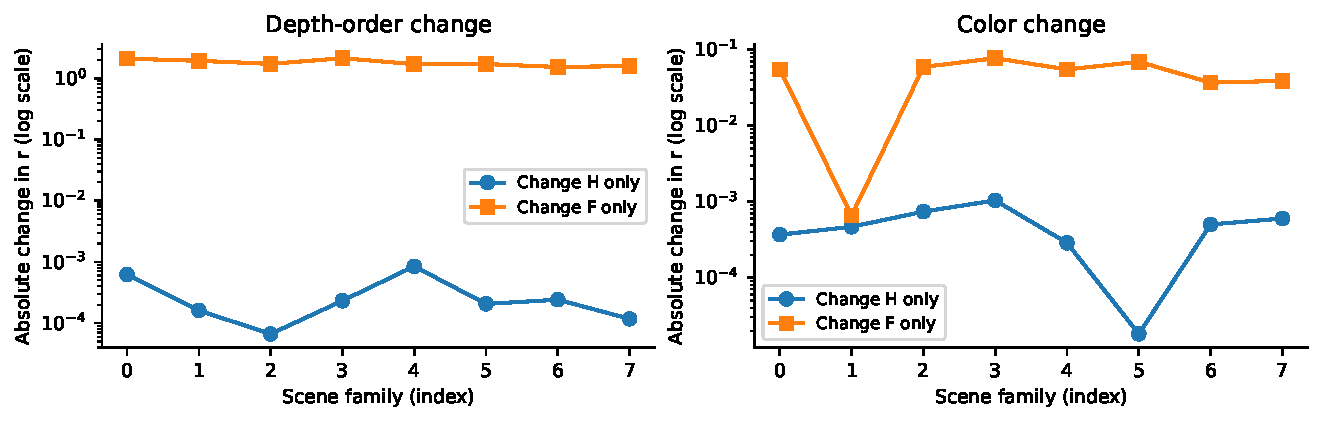
\includegraphics[width=\linewidth]{factorial.pdf}
\caption{E1 on archived FP32 pairs. Horizontal axis: scene-family index within each comparison. Vertical axis: absolute change in calibrated relation score $r$, on a logarithmic scale. Circles change CoVT states $H$ while holding expert features fixed; squares change expert features $F$ while holding states fixed. Left: depth swaps; right: color changes. Lines connect families for readability, not a time series. No confidence bands are shown.}\label{fig:factorial}
\end{figure}
\takeaway{Expert features carry the dominant measured depth-order change into this readout. This does not yet tell us what the answer computation uses.}

\subsection{Can the same states work for different images?}
\textbf{Purpose and design.} Test whether successful depth readout requires image-specific states. Retain each target's expert features but replace its states with a fixed mean, a fixed example, or states from another image. Shuffle the order of the four CoVT states while retaining expert features, testing the state-to-expert-level assignment. Zero-state and zero-projection controls are audited separately.

\textbf{Example.} Use exactly the same four state vectors for a scene where A is nearer and another where B is nearer. If both maps are correct, their distinction must be supplied by something that still varies, such as expert features.

\textbf{Results.} Native, fixed, and cross-image state conditions all achieved 100\% relation accuracy on the 32-image follow-up. State-order shuffle averaged 58.125\% across five repeats; both zero controls abstained on all images. In the 200-image geometry-shift batch, fixed-state readout was correct on 199/200 with one abstention; the expert was correct on 198/200 with two abstentions. In a selected 40-image native-generation subset, 39 yielded the required states and text was correct on 22/40. On eligible examples, native and fixed-state predictions agreed, with 38/39 correct; the shuffled-state family mean was 56.5\%.
\takeaway{Fixed states remain useful across these synthetic settings. The assignment of states to expert feature levels matters in the tested readout. The result concerns this conditional decoder, not a universal claim that CoVT states contain no information.}

\subsection{Could wording or letter recognition explain the gap?}
\textbf{Purpose and design.} Use the eight prompts and image variants in Section~3 to separate technical wording, letter recognition, size judgment, and depth consistency. Compare CoVT with its Qwen base model on the same 16 images, without filtering for initial correctness.

\textbf{Example.} After swapping only the printed A and B labels, a correct near answer should change letters while preserving the selected physical point. If the model reads the letters correctly but fails this paired test, simple letter blindness is an incomplete explanation.

\textbf{Results.} Both models scored 16/16 on left-label and apparent-area questions. Plain-near wording gave 11/16 for each; the original wording gave 6/16 for CoVT and 8/16 for the base model. Both changed letters as expected on only 3/8 label-swap pairs. Near/far answers were complementary on 9/16 CoVT images and 10/16 base images. Complementarity is a consistency measure; two complementary answers can still both disagree with the corresponding truth. Figure~\ref{fig:prompts} includes all eight conditions.
\begin{figure}[htbp]\centering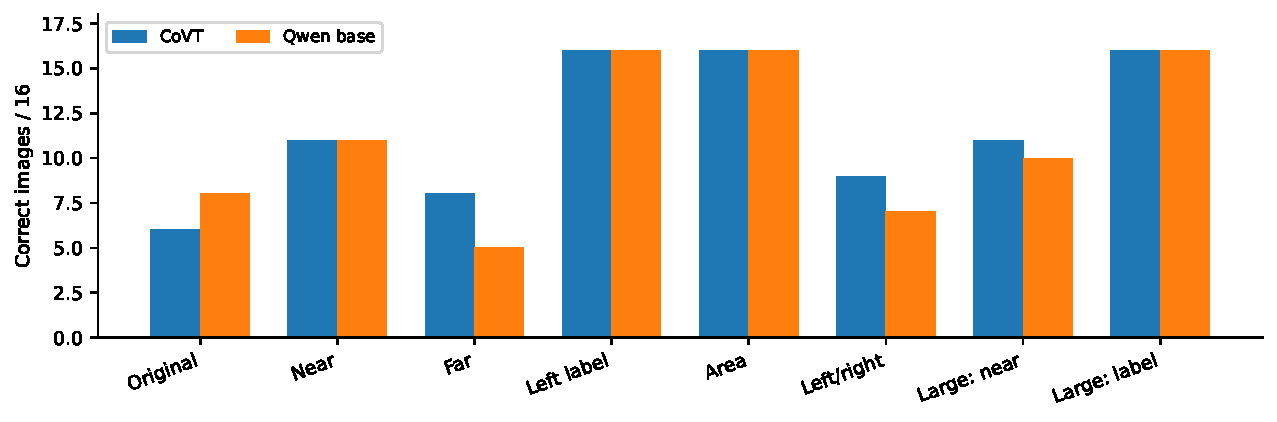
\includegraphics[width=\linewidth]{prompts.pdf}
\caption{Answer diagnostics. Horizontal axis: the eight conditions defined by the exact prompts in Section~3; ``Large'' means enlarged printed labels. Vertical axis: correctly answered images out of 16 per task and model. Colors compare CoVT and the Qwen base model. Repeated bars reuse the same eight scene families; they are not independent datasets.}\label{fig:prompts}
\end{figure}
\takeaway{Simpler wording helps on these examples, but label recognition and wording do not explain all depth errors. This comparison does not isolate which part of CoVT training caused any difference.}

\subsection{Does the model simply select the larger object?}
\textbf{Purpose and design.} The larger-object rule succeeds on 84\% of the 200-image shift batch and 92.5\% of its selected 40-image subset, so that batch alone is insufficient to exclude a size shortcut. We therefore use eight families with four variants each, crossing nearer label A/B with whether apparent size agrees or conflicts with depth. There are 16 images in each size condition and 16 for each correct label.

\textbf{Example.} In one image A is nearer and looks larger; in its controlled counterpart A remains nearer but looks smaller. A rule that always chooses the larger object cannot answer both correctly. Physical-size adjustments used to create this control may also change other cues, so the control is not a complete isolation of every visual feature.

\textbf{Results.} Text accuracy was 25/32, including 12/16 size-agreement and 13/16 size-conflict cases. Fixed-state depth was 30/32 (16/16 and 14/16); expert depth was 26/32 (16/16 and 10/16). See Fig.~\ref{fig:balanced}.
\begin{figure}[htbp]\centering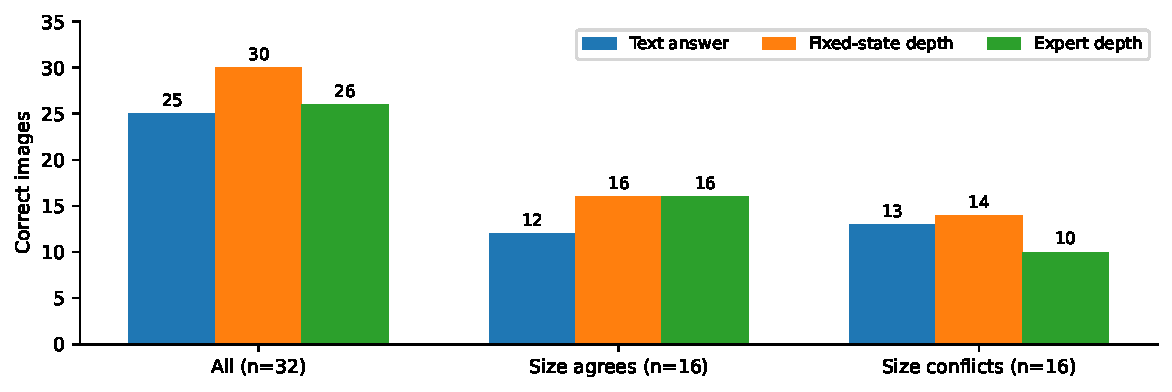
\includegraphics[width=.94\linewidth]{balanced.pdf}
\caption{Size-balanced results. Horizontal groups distinguish all images, apparent-size agreement, and apparent-size conflict; denominators are printed below each group. Vertical axis: correct-image count. Colors distinguish text answers, fixed-state depth readout, and expert depth. The total group includes the two subgroups and must not be counted as additional data.}\label{fig:balanced}
\end{figure}
\takeaway{Always choosing the larger object cannot explain all successful answers here. The experiment does not prove that answers rely on the four depth states.}

\subsection{Do interventions inside the language model change answers?}
\textbf{Purpose and design.} Move beyond decoder-only edits. Replace intermediate vectors at selected depth-token positions with vectors from a donor image, then recompute downstream answer generation. A donor is another recorded example; an opposite-depth donor has the opposite near label. Same-depth donors, shuffled donors, identity replacement, and an answer-readout positive control test alternative effects and the measurement apparatus.

Of the 32 balanced images, 26 naturally generated four depth pads; 20 targets from six families met the opposite-depth pairing requirements. Initial natural-state interventions showed no flips in tested opposite-depth, same-depth, and shuffled conditions. A subsequent scan used zero-based layers 0, 4, 8, 14, 20, 24, and 27. There were 140 opposite-depth interventions and 140 zero interventions, plus 140 identity checks and 20 answer-readout positive controls.

\textbf{Example.} Keep an A-near target image visible, replace one layer's four depth-position states with those from a B-near donor, and let the model continue. A resulting B would show sensitivity to the intervention; because the original image still supports A, it would not automatically be an accuracy improvement.

\textbf{Results.} All 140 natural opposite-depth interventions left the answer unchanged; the largest absolute probability change was about 0.00710 percentage points. Identity and answer-readout controls passed. Zeroing produced a different phenomenon: at layers 4, 8, 14, and 24, none of the 20 outputs had an unambiguous valid answer. At layer 20 only 3/20 were valid and unchanged; at layers 0 and 27 all 20 were valid and unchanged. Malformed tags, ambiguity, and early termination are not successful depth transfer.
\takeaway{These natural single-layer substitutions did not control answers. Zeroing can disrupt output structure, which must be distinguished from a task-relevant answer change.}

\subsection{Was one layer or four positions too little?}
\textbf{Purpose and design.} Increase coverage to five settings: early layers 0--8, middle 9--17, late 18--27, all 28 layers, and all layers over the 15 positions of the tested thought block. Twenty targets and opposite/same-depth donors give 200 interventions, with 100 identity controls. These conditions still do not patch all image, question, or answer positions.

\textbf{Results.} All 200 interventions preserved the full generated token sequence and valid answers. All 100 identity controls were exact. In the widest condition, the maximum absolute opposite-depth probability effect was 0.047183 percentage points; the same-depth maximum was about 0.0422. The family-mean opposite-minus-same directional effect was approximately 0.00377 percentage points, with interval $[-0.00573,0.0136]$, including zero.

\textbf{Actual example.} For target \texttt{balanced\_003\_d1\_s0} and its opposite-depth donor \texttt{d0\_s0}, $q_A$ moved from 0.84342670 to 0.84295487. The decrease is 0.047183 percentage points, and the generated answer remained A. Six targets had opposite-depth donors with a different natural answer; none flipped in the audited comparison.
\takeaway{Expanding these layer and position ranges did not reveal answer control. This bounds the tested intervention family; it neither proves exact equivalence nor rules out information traveling through unpatched positions.}
\FloatBarrier

\section{What the results establish, and what remains open}
The strongest evidence concerns the visualization branch. Its depth ordering is highly sensitive to expert-feature changes, and fixed states often suffice when paired with target expert features. The text branch behaves differently under our tested state substitutions. These observations are consistent with substantial expert support for visualization and an answer computation that can use other information, but they do not uniquely identify a mechanism.

Several explanations remain viable. Information may already have moved from the depth positions into other positions before a tested intervention. The answer may rely on direct or indirect image information. The transplanted states may fail to replace the relevant semantic quantity even when shapes and indices match. A model may also reasonably retain an answer supported by the target image when contradictory donor states are injected. Redundant paths can further reduce the effect of a single intervention family.

The experiment is not inherently limited to depth. CoVT includes other visual supervision types, and segmentation could provide another controlled question, such as which labeled point belongs to an object region. That extension requires a compatible checkpoint and decoder, region-level scoring, and new controls. The current depth results cannot be transferred to segmentation without running those tests.

\textbf{Scope and novelty.} We have tested one released depth checkpoint on small, related synthetic batches. We have no natural-image validation, confirmed path localization, or repair result. The first proposal's literature audit already identifies prior work on visual-state utilization and token replacement; generic statements that a state can be unused are insufficient novelty claims. A stronger contribution would identify a particular computation, show how a controlled edit affects both outputs, and explain a reproducible class of ordinary errors.
\takeaway{The project has a reproducible diagnostic basis. Its central causal question remains unresolved, which determines the revised next steps.}

\section{Revised research plan}
The first proposal's central idea remains useful: intervene at a \emph{shared upstream computation} and recompute both downstream outputs. If we edit only the map decoder after the language model has already produced its states, the text answer has no reason to change. Conversely, an intervention that changes both outputs is interpretable only when we track what else changed and whether the result follows the intended relation.

\begin{enumerate}[leftmargin=*]
\item \textbf{Test currently uncovered positions.} Examine the transition text between the visual thought and answer, then selected question and image positions. Keep the target input fixed. Compare opposite-depth, same-depth, identity, and nuisance donors. Record both free generation and any fixed-continuation probability measurement. Continue only if a normal, task-related effect is reproducible beyond matched controls.
\item \textbf{Recompute both outputs from the same edit.} At an audited shared upstream site, recompute the resulting four states, depth map, and answer. Record which expert features are held fixed. For example, a B-readout with an unchanged A answer after injecting B-donor content demonstrates different responses to that operation; it does not, without further evidence, diagnose a faulty reader.
\item \textbf{Locate the information path.} Distinguish information passed through visual-thought positions from information reaching the answer through other positions. Blocking a direct image-to-answer link may leave image information already copied into text positions. Select candidate components on discovery families and validate the proposed path on new families and donors.
\item \textbf{Attempt repair only after localization.} First check whether a diagnostic replacement with appropriate information can improve a defined error class. Such a replacement is an oracle test if it uses extra correct information. Only then consider a small trainable update to localized answer components. Compare against ordinary fine-tuning and random-component updates with matched data and parameter budgets.
\item \textbf{Confirm outside the discovery data.} Freeze the protocol before testing new scene families, richer geometry, natural images, or another checkpoint. A segmentation extension is a separate replication. Its labels and measurement assumptions must be established independently.
\end{enumerate}

We remove the original proposal's premature choices of repair component counts, update ranks, and training-scene budgets from the active plan. We also remove any framing that presupposes a defective answer reader or treats map--answer disagreement as a sufficient mechanism claim. Training scale and stopping criteria should follow a localized effect and its variance, not precede it.

Discovery, validation, and final confirmation must split by scene family. Reused donors introduce additional dependence and should be addressed through disjoint pairings or an appropriate dependence-aware analysis. A claim of practical equivalence requires a prespecified tolerance and an interval contained within that tolerance; zero observed flips alone does not suffice.

\begin{table}[htbp]\centering\small
\begin{tabularx}{\linewidth}{lYY}\toprule
Original stage & Goal & Status after this pilot\\\midrule
E0 & Recover and calibrate native readout & Completed for audited batches.\\
E1 & Separate state and expert inputs & Completed as a small-scale diagnostic.\\
E2 & Shared-upstream semantic intervention & Partial: internal scans completed; joint causal interpretation unresolved.\\
E3 & Locate answer and visual information paths & Not completed.\\
E4 & Compare sensitive directions, then validate finite edits & Not executed.\\
E5 & Repair a localized error mechanism & Not executed; evidence gate unmet.\\\bottomrule
\end{tabularx}\caption{The revised plan distinguishes completed diagnostics from intended causal and repair contributions.}
\end{table}
\takeaway{The next useful result is a reproducible, well-formed, task-related intervention effect and a verified information path. Further broad scans or repair training are not yet justified by a localized mechanism.}

\appendix
\section{Reproducibility and provenance}
These notes consolidate \texttt{dual\_readout\_proposal.tex} with the archived experiment report and source code. The second proposal, concerning reusable query states, remains a separate direction. Model runs were performed remotely in Colab; document preparation only reads saved artifacts.

The audited implementation uses \texttt{transformers==4.50.1}, eager attention, deterministic generation, and depth token ID 151669. The restoration code requires exactly four naturally generated depth pads. Its state semantics are post-final-normalization values at depth-pad input positions, without a one-token shift. Exact checkpoint revisions, projection files, configuration settings, and per-image outputs are retained in the run records. FP32 results should not be silently combined with the initial BF16 eligibility failures.

\begin{table}[htbp]\centering\footnotesize
\begin{tabularx}{\linewidth}{lY}\toprule
Evidence & Run directory suffix within \texttt{covt-pilot/runs}\\\midrule
Initial restoration & \nolinkurl{colab-20260918-backup/runs/colab-e0-20260918-032255}\\
FP32 / E1 & \nolinkurl{colab-20260918-followup/runs/followup-fp32-20260918-043002}\\
Answer diagnostics & \nolinkurl{colab-20260918-answer-shift/extracted/runs/answer-diagnostic-20260918-050133}\\
Geometry shift & \nolinkurl{colab-20260918-answer-shift/extracted/runs/shift-validation-20260918-050713}\\
Balanced / initial interventions & \nolinkurl{colab-20260918-balanced-intervention/extracted/runs/balanced-intervention-20260918-090000}\\
Layer scan & \nolinkurl{colab-20260918-layer-scan/extracted/runs/layer-scan-20260918-093053}\\
Block scan & \nolinkurl{colab-20260918-block-intervention/extracted/runs/block-intervention-20260918-100708}\\\bottomrule
\end{tabularx}\caption{Evidence index. Tables and plots summarize these saved runs; run counts are not independent scene counts.}
\end{table}

Question construction is in \nolinkurl{src/covt_pilot/scenes.py}, \texttt{shift\_scenes.py}, and \texttt{diagnostics.py}; input templating and extraction are in \texttt{model.py}; relation scoring is in \texttt{metrics.py}. English plots are regenerated from saved records by \texttt{scripts/build\_notes\_figures.py}. The separate offline dataset gallery in the repository contains the same 284 image records. Original-paper figure provenance is recorded in \texttt{output/html/paper\_figures/provenance.json}. Rights to reproduced paper figures remain with the original authors.

\begin{thebibliography}{9}
\bibitem{covt} Yiming Qin et al. \emph{Chain-of-Visual-Thought}. Official paper and released implementation. \url{https://wakalsprojectpage.github.io/covt-website/static/pdf/paper.pdf}; \url{https://github.com/Wakals/CoVT}.
\bibitem{dav2} Lihe Yang et al. \emph{Depth Anything V2}. 2024. \url{https://arxiv.org/abs/2406.09414}.
\end{thebibliography}
\end{document}
